\chapter{The Theory behind Machine Learning}
\label{ch:neural-network}

In this Chapter we will see how machine learning techniques can be successfully applied to solve financial problems. We first do a quick tour on the theory behind neural networks and then see few examples and practical applications regarding regression and classification issues.

Beware that this Chapter just scratches the surface of machine learning theory which has seen a huge development in the latest years leading to thousands of applications in many different fields.
    
\section{Neural Networks}\label{neural-networks}

Artificial Neural Networks (ANN or simply NN) are information processing models that are developed by inspiring from the working principles of the human brain. Their most essential property is \emph{the ability of learning from sample sets}.

\subsection{Neurons and Activation Functions}
The basic unit of an ANN is the neuron.
It consists of weights (\(w_i\)) and takes in input real numbers (\(x_i\)). After the injection into a neuron all these inputs are individually weighted, added together (sometimes it is added also a bias \(w_0\)) and passed into the activation function which produces the final neuron output

\[ \textrm{Inputs} = \sum_{i=1}^{N} x_i w_i + w_0 \rightarrow f(\textrm{Inputs}) = \textrm{Outputs}\]
Figure~\ref{fig:neuron} shows an example.

There are many different types of activation functions, examples are
\begin{itemize}
\item \emph{step function}: which returns just 0 or 1 according to the input value;
\item \emph{sigmoid}: which can be thought of as the continuous version of the step function, see Fig.~\ref{fig:act_func};
\item \emph{Rectified Linear Unit} (ReLU);
\item \emph{hyperbolic tangent} (tanh).
\end{itemize}

For a deeper discussion on activation functions see~\cite{bib:activation_function}.

\begin{figure}[htb]
\centering
\subfloat[Model of an artificial neuron.\label{fig:neuron}]{%
	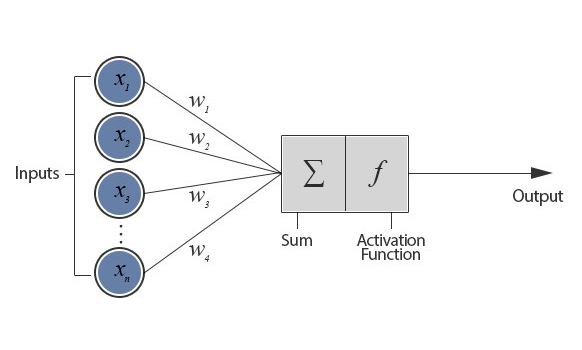
\includegraphics[width=0.6\textwidth]{figures/neuron}
}
\subfloat[Examples of sigmoidal and step activation functions.\label{fig:act_func}]{%
	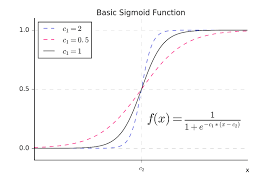
\includegraphics[height=0.30\textwidth]{figures/sigmoid}
}
\caption{Basic components of a neuron.}
\label{fig:sigmoid}
\end{figure}

\subsection{Training of a Neuron}
\label{training-of-a-neuron}

When teaching children how to recognize a bus, we just tell them, showing an example: "This is a bus. That is not a bus." until they learn the concept of what a bus is. Afterwards, if a child sees new objects that she hasn't seen before, we could expect her to recognize correctly whether the new object is a bus or not.

This is exactly the idea behind neuron training. Inputs from a \emph{training} set are presented to the neuron,  one after the other, together with the correct output. During the process neuron weights are modified so that its response best matches the true output.

When an entire pass through all of the inputs is completed (an \emph{epoch}) the neuron has learned. Usually to make it learn even better the same training data is processed multiple times.

After the training is completed, when an input vector \(\mathbf{x}\), contained in the training set, is presented to the neuron, it will output the correct value. If \(\mathbf{x}\) is not in the training set, the neuron will respond with an output close to those corresponding to other training vectors similar to \(\mathbf{x}\).

This kind of training is called \emph{supervised} because the input dataset is accompanied by the known targets (the true outputs), and we want our model to learn to predict the target from those input variables.

Unfortunately using just a neuron is not too useful since with such a simple architecture is not possible to solve the interesting problems we would like to face. 
The next step is to put together more neurons in \emph{layers}.

\subsection{Multilayered Neural Networks}
\label{multi-layered-neural-networks}

In a multilayered configuration each neuron from the \emph{input layer} is fed up to each node in the next \emph{hidden layer}. This kind of connection is repeated for each node down to the \emph{output layer}. 
We should note that there can be any number of nodes per layer and there are usually multiple hidden layers to pass through before ultimately reaching the output layer. The only two architectural constraints are on the neuron number in the input layer, that has to match the number of inputs, and on the nodes in the output layer which depends on the kind of target. Figure~\ref{fig:multilayered_nn} shows an example of such an architecture.

\begin{figure}[htb]
\centering
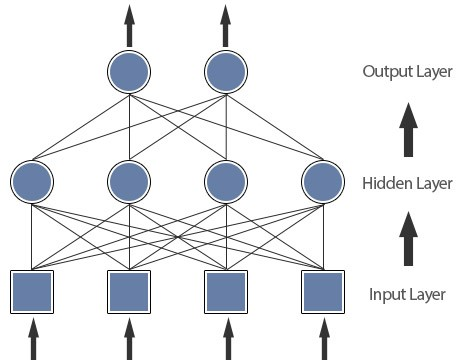
\includegraphics[width=0.6\textwidth]{figures/multilayer.jpeg}
\caption{A multilayered neural network.}
\label{fig:multilayered_nn}
\end{figure}

\subsection{Training a Multilayered Neural Network}
\label{training-a-multilayered-neural-network}

The training of a multilayered NN follows these steps:

\begin{itemize}
\tightlist
\item present an input sample to the neural network whose neurons are initialized with random weights;
\item compute the network output obtained by calculating the activation functions of each layer;
\item calculate the \emph{error (loss)} as the difference between NN predicted and target output;
\item re-adjust the network weights such that the error decreases;
\item continue the process for the entire sample (and also for several epochs), until the error is not changing too much (i.e. the process converged).
\end{itemize}
In Figure~\ref{fig:training} an example of training is shown.

\begin{figure}[htb]
\centering
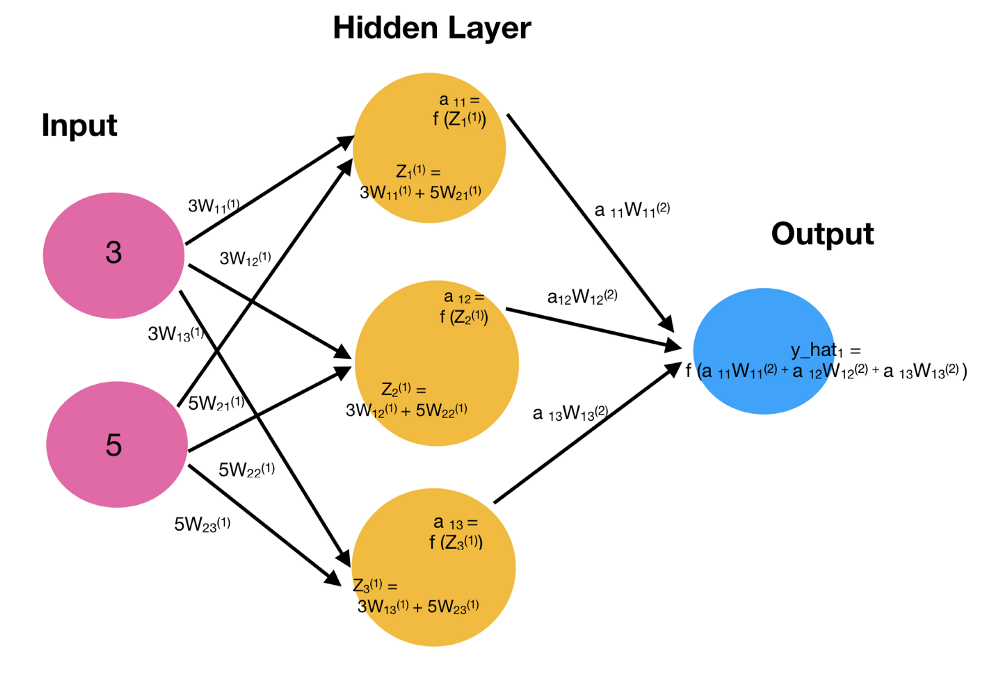
\includegraphics[width=0.9\textwidth]{figures/training_nn}
\caption{Training example of a multilayered neural network.}
\label{fig:training}
\end{figure}

\subsubsection{Loss Function}
The NN error is computed by the \emph{loss function}. Different loss functions will give different error estimates for the same prediction, and thus they have a considerable effect on the performance of any model. Two are the main choices

\begin{itemize}
\tightlist
\item Mean Absolute Error (MAE): the average of the absolute value of the differences between the predictions and true values. It shows how far off we are on average from the correct value. 
\item Root Mean Squared Error (MSE): the square root of the average of the squared differences between the predictions and true values. It instead penalizes larger errors more heavily and is commonly used in regression tasks. 
\end{itemize}

Either metrics may be appropriate depending on the situation and you can use both for comparison. 
More information about loss function can be found in~\cite{bib:loss_function}.

\subsubsection{Back-propagation}
The loss is a function of the internal parameters of the model (i.e neuron weights). For an accurate predictions, one needs to minimize the calculated error and in a neural network, this is done using
\emph{back-propagation}~\cite{bib:backpropagation}.

In this algorithm the current error is "propagated" backwards to previous layers, where it is used to modify the weights in such a way that the loss tends to be minimized.
The weights are modified with a function called \emph{optimization function} (we will use \emph{Adam} in the following but there are more).

\subsection{Regression and Classification}
\label{regression-and-classification}

The two main categories of problems that can be solved with neural networks are \emph{classification} and \emph{regression}. Let's see their characteristics and differences.

\subsubsection{Classification}
\label{classification}

Classification is the process of finding a function which helps in dividing the input dataset into classes based on its characteristics. 
The goal is to find the mapping function between the input (\(x\)) and the \textbf{discrete} output (\(y\)) or in other words to find the decision boundary, which can divide the dataset into the different classes.

A typical classification problem is the \emph{email spam detection}. The model is trained on different parameters using millions of emails, and whenever it receives a new email, it checks whether is spam or not. Classification algorithms can also be used in speech recognition, car plates identification, \ldots

\subsubsection{Regression}
\label{regression}

Regression is the process of finding hidden correlations between dependent variables. It helps in predicting market trends, house prices, \ldots

The goal is to find the mapping function between the input variables (\(x\)) and the \textbf{continuous} output variable (\(y\)), that is to find the best fit which can predict the output.

As an example suppose we want to do weather forecasting. The model is trained on past data, and on the basis of today's inputs can predict the weather for future days. In general whenever we are dealing with function approximations this kind of algorithms can be applied.

\begin{attention}
\subsubsection{Technical Note}
\label{technical-note}

Neural network training and testing is performed using two modules: \texttt{keras}~\cite{bib:keras} (which in turn is based on a Google open source library called \texttt{tensorflow}~\cite{bib:tensorflow}) and \texttt{scikit-learn}~\cite{bib:scikit} which provide many useful utilities.
\end{attention}

\section{Function approximation}
\label{function-approximation}

Let's design an ANN which is capable of learning the functional form underlying a set of data. 

The training sample is generated as a two columns array: \(x\) (input), \(f(x)\) (target output) where \(f(x) = x^3 +2\). 

Before embarking into the actual training the sample undergoes to a transformation in order to have all the inputs (and outputs) with the same scale. This sample transformation is called \emph{scaling}, and is done to provide the NN with "equalized" inputs since it could be fooled by very large or small numbers giving unstable results.

There are various methods available for data scaling in \texttt{scikit-learn}, the most important being:
\begin{itemize}
\tightlist
\item \emph{StandardScaler}: scales features such that the distribution is centered around 0, with a standard deviation of 1. It is not quite good if data is not normally distributed (i.e. no Gaussian distribution);
\item \emph{MinMaxScaler}: shrinks the range such that it becomes between 0 and 1 (or -1 to 1 if there are negative values in the first place). It is influenced heavily by outliers (i.e. extreme values);
\item \emph{RobustScaler}: similar to the previous one but it instead uses quantile ranges, so that it is robust against outliers. It doesn't take the median of the original sample into account and only focuses on the regions where the bulk data is. Consider that \textbf{robust} doesn't mean immune or invulnerable and that the purpouse of scaling is not to remove outliers.
\end{itemize}

Which one to use depends on the particular case under study. 

\begin{ipython}
import numpy as np
X = np.array([(x, x**3+2) for x in np.arange(-2, 2.001, 0.001)])
print("Distribution of original data ", X[:, 0].min(), X[:, 0].max(), 
X[:, 1].min(), X[:, 1].max())
\end{ipython}
\begin{ioutput}
Distribution of original data  -2.0 1.999999999995595 -6.0 9.99999999994714
\end{ioutput}

Figure~\ref{fig:scalers} reports the different transformations on the distribution of the target outputs. In the actual example we are going to use the \texttt{MinMaxScaler}.

\begin{figure}[htb]
\centering
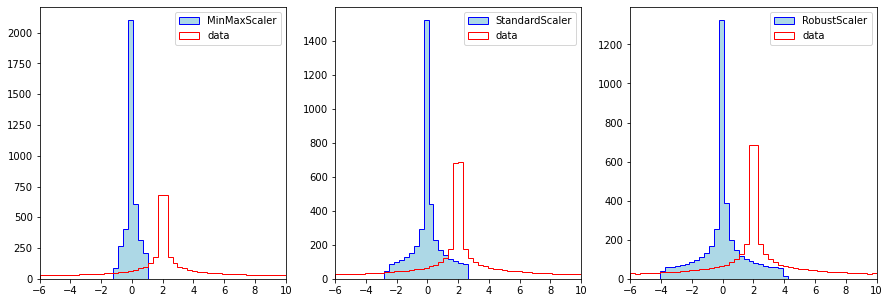
\includegraphics[width=0.9\textwidth]{figures/scalers}
\caption{Effect of different kind of scalers in the target output distribution.}
\label{fig:scalers}
\end{figure}

\begin{ipython}
from sklearn.model_selection import train_test_split
from sklearn.preprocessing import MinMaxScaler

scale = MinMaxScaler(feature_range=(-1,1))
X_scaled = scale.fit_transform(X)

print("The same data after the normalization ", X_scaled[:, 0].min()
                                              , X_scaled[:, 0].max()
                                              , X_scaled[:, 1].min()
                                              , X_scaled[:, 1].max())

X_train, X_test = train_test_split(X_scaled, test_size=0.2)
\end{ipython}
\begin{ioutput}
The same data after the normalization  -1.0 1.0 -1.0 1.0
\end{ioutput}

Notice that the sample has been split into two parts: training and testing. The reason will be explained in Sec.~\ref{sec:overtraining}.

\subsection{Neural Network Design}
\label{neural-network-design}

There is no rule to guide developers into the design of a neural network in terms of number of layers and neurons (the so called \emph{hyper-parameters}). 

One popular method for hyper-parameter optimization is the \emph{grid search}. 
A list of possible values for each hyper-parameter is defined, then the model is run multiple times, each time with a different combination of the hyper-parameter values. In the end the set giving the best result is taken. This is the most thorough way of selecting the neural network architecture but it is also the most computationally intense.
In the end a \emph{trial and error} strategy is what is implemented anyway, and the solution giving the best accuracy is selected although without an exhaustive check of all the possibilities.

In general a larger number of nodes is better to catch highly structured data with a lot of feature although it may require larger training sample to work correctly.

As a rule of thumb a NN with just one hidden layer with a number of neurons averaging the inputs and outputs is sufficient in most cases.

In the following we will use complex networks just for illustration, but no attempt in optimizing the layout has been done at all.

Here two layers with 15 and 5 neurons respectively and a \texttt{tanh} activation function are used, see Fig,~\ref{fig:ann_1}. The \texttt{inputs} parameter has to be set to 1 since we have just one single input, the \texttt{x} value.

\begin{ipython}
from keras.models import Sequential
from keras.layers import Dense

x = X_train[:, 0]
y = X_train[:, 1]
model = Sequential()
model.add(Dense(15, input_dim=1, activation='tanh'))
model.add(Dense(5, activation='tanh'))
model.add(Dense(1, activation='tanh'))

model.compile(loss='mse', optimizer='adam')
model.fit(x, y, epochs=2000, verbose=1)
\end{ipython}
\begin{ioutput}
Epoch 1/2000
100/100 [==============================] - 1s 2ms/step - loss: 0.0362
Epoch 2/2000
100/100 [==============================] - 0s 2ms/step - loss: 0.0293
...
Epoch 1999/2000
100/100 [==============================] - 0s 2ms/step - loss: 5.6730e-06
Epoch 2000/2000
100/100 [==============================] - 0s 3ms/step - loss: 6.1324e-06
<keras.callbacks.History at 0x7f9c22abd450>
\end{ioutput}

\begin{figure}[htb]
\centering
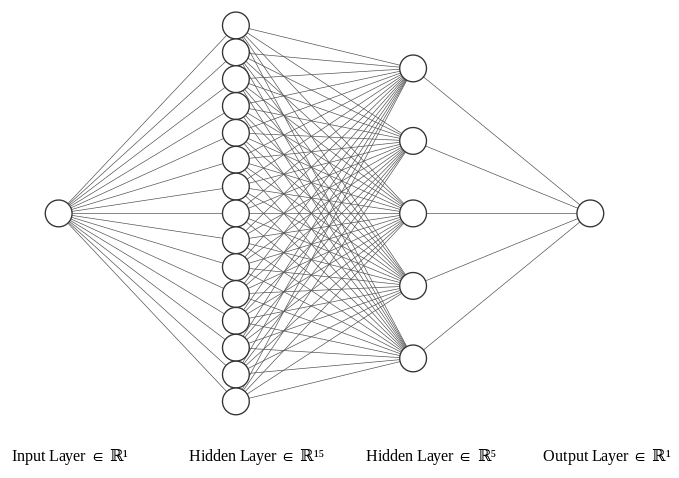
\includegraphics[width=0.9\textwidth]{figures/ann_1.png}
\caption{Graphical representation of the ANN used to approximate the function $f(x) = x^3 + 2$.}
\label{fig:ann_1}
\end{figure}

The output shows a counter with the current epoch number and the computed loss which is evaluated using the method chosen in the code.
When the training is completed we can evaluate how good it is. \textbf{Usually performance is measured using the loss function value at the end of the training.}

Since it takes some time to generate data samples, it is always advisable to save them in a file since it may be needed to load it many times during the NN development. 
Also both the training model and the actual scalers need to be stored in files in order to use them for prediction. Indeed the NN has to work with "similar" data used during the training so the same scaling functions need to be applied.

\begin{ipython}
import joblib

job_name = 'func_approx'
model.save(job_name)
joblib.dump(scale_X, job_name + "_x_scaler.save")
joblib.dump(scale_Y, job_name + "_y_scaler.save")
\end{ipython}

\subsection{Model Prediction}

A \emph{perfect} prediction would lead to \(\textrm{loss}=0\) so the lower these numbers the better is our training. 

Model performance improves with the number of epochs in the training, since the NN has more chances to learn the input features. To get an idea of what is going on in Fig.~\ref{fig:training_vs_epochs} are shown the actual function we want to approximate and different predictions obtained with the same NN architecture but various number of epochs (i.e. 5, 100, 800, 5000) in the training.

\begin{figure}[htb]
\centering
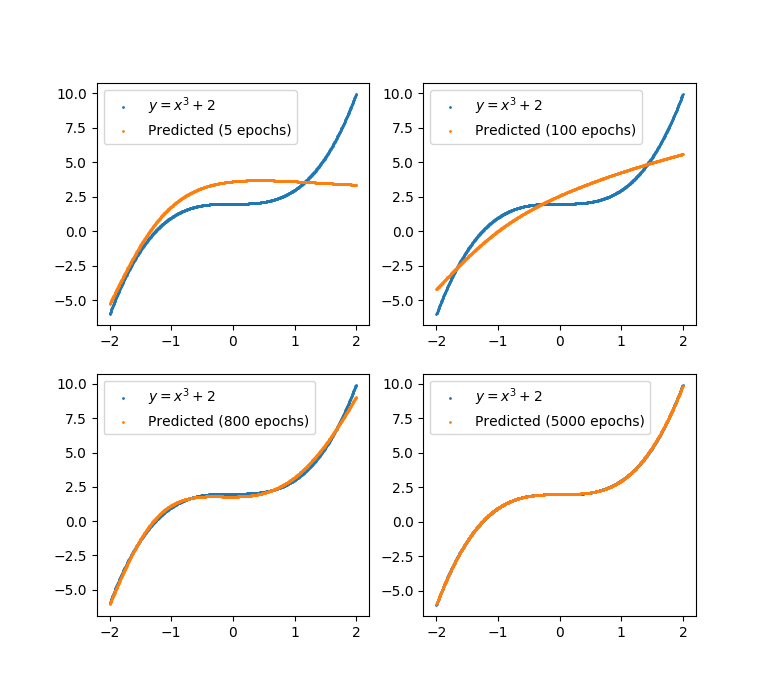
\includegraphics[width=0.9\textwidth]{figures/training_vs_epoch}
\caption{Prediction of the target $f(x)$ using different number of epochs in the training (5, 100, 800 and 5000) respectively.}
\label{fig:training_vs_epochs}
\end{figure}

\subsection{Overtraining}
\label{sec:overtraining}
A common issue to avoid during the training is \emph{overtraining} or \emph{overfitting} a NN. 

This happens when a model is "trained too well" on the dataset. This means that the model mostly memorized data, and its performance accounts for a large accuracy within it but a low accuracy in similar but independent datasets. 

To check for overfitting it is required to split the available sample in at least two parts: training and testing (e.g.~80\% and 20\%) and to use the former to perform the training and the latter to cross-check the performance.

%Actually you should split the sample in three parts: training, testing and validation. What you would do is take the model with the highest validation accuracy and then test it with the testing set.
%This makes sure that you don’t overfit the model. Using the validation set to choose the best model is a form of data leakage (or “cheating”) to get to pick the result that produced the best test score out of hundreds of them. Data leakage happens when information outside the training data set is used in the model.
%In this case, our testing and validation set are the same, since we have a smaller sample size.

Looking at the output of the \texttt{evaluate()} calls we can compare the loss computed with the training sample to that on the testing sample. If the two numbers are comparable the NN is ok, otherwise if the loss on the training is much smaller than the testing we had overfitting.
In our example since the two numbers are in good agreement we can be confident that there hasn't been overtraining.

The check can be done with the \texttt{evaluate()} method

\begin{ipython}
eval1 = model.evaluate(X_train[:, 0], X_train[:, 1])
print('Training: {}'.format(eval1))

eval2 = model.evaluate(X_test[:, 0], X_test[:, 1])
print('Test: {}'.format(eval2))
\end{ipython}
\begin{ioutput}
100/100 [==============================] - 0s 1ms/step - loss: 5.2089e-06
Training: 5.208917627896881e-06
26/26 [==============================] - 0s 2ms/step - loss: 5.2780e-06
Test: 5.277975560602499e-06
\end{ioutput}

In case one would need more accuracy and had already incremented too much the number of epochs could either increase the training sample size or change the NN architecture.

\subsection{Why Am I Getting Different Results ?}

This is to be expected and might even be a feature of the algorithm, not a bug.

In applied machine learning, we run a machine learning “algorithm” on a dataset to get a machine learning “model.” The model can then be evaluated on data.
We cannot write code to predict outputs given inputs because it is too hard, so we use machine learning algorithms to learn how to predict outputs from inputs given historical examples.
Unlike the programming that we may be used to, the programs may not be entirely deterministic.

The resulting machine learning models may be different each time they are trained. In turn, the models may make different predictions, and when evaluated, may have a different level of error or accuracy.

\subsubsection{Differences in Training Data}

You will get different results when you run the same algorithm on different data.

The variance is a measure of how sensitive the algorithm is to the specific data used during training.

\subsubsection{Stochastic Learning Algorithm}

You can get different results when you run the same algorithm on the same data due to the nature of the learning algorithm.

Some machine learning algorithms are deterministic. Just like the programming that you’re used to. That means, when the algorithm is given the same dataset, it learns the same model every time. An example is a linear regression or logistic regression algorithm.

Some algorithms are not deterministic; instead, they are stochastic. This means that their behavior incorporates elements of randomness.

Stochastic does not mean random. Stochastic machine learning algorithms are not learning a random model. They are learning a model conditional on the historical data you have provided. Instead, the specific small decisions made by the algorithm during the learning process can vary randomly.

The impact is that each time the stochastic machine learning algorithm is run on the same data, it learns a slightly different model. In turn, the model may make slightly different predictions, and when evaluated using error or accuracy, may have a slightly different performance.

Neural networks are a stochastic machine learning algorithm. The random initial weights allow the model to try learning from a different starting point in the search space each time and allow the learning algorithm to “break symmetry” during learning. The random shuffle of examples during training ensures that each gradient estimate and weight update is slightly different.

Nevertheless the randomness used by learning algorithms can be controlled. For example, you set the seed used by the pseudorandom number generator to ensure that each time the algorithm is run, it gets the same randomness.

This is not a good approach in practice (apart from tutorials or lectures). Since there is no best seed for a stochastic machine learning algorithm you can summarize the performance of these models by fitting multiple final models on your dataset and averaging their predictions.

\subsubsection{Evaluation Procedure}
You can get different results when running the same algorithm with the same data due to the evaluation procedure.

A train-test split involves randomly assigning rows to either be used to train the model or evaluate the model to meet a predefined train or test set size.

\subsubsection{Differences Caused by Platform}
You can get different results when running the same algorithm on the same data on different computers.

This can happen even if you fix the random number seed to address the stochastic nature of the learning algorithm and evaluation procedure.

The cause in this case is the platform or development environment used to run the example, and the results are often different.

Some of the possible causes are:
\begin{itemize}
\tightlist
\item system architecture, e.g. CPU or GPU;
\item operating system, e.g. MacOS or Linux;
\item underlying math libraries, e.g. LAPACK or BLAS;
\item Python of library version, e.g. 3.6 or 3.7, scikit-learn 0.22 or 0.23.
\end{itemize}

Honestly, the effect is usually very small in practice (at least in my experience) as long as major software versions are a good or close enough match.

\section{Image Recognition Neural Network}
\label{neural-net-to-recognize-handwritten-digits}

The difficulties of visual pattern recognition becomes immediately apparent if you attempt to write a computer program to recognize digits like those in Fig.~\ref{fig:mnist}.

\begin{figure}[b]
\centering
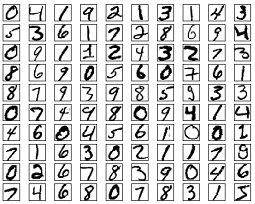
\includegraphics[width=0.5\textwidth]{figures/mnist_100_digits}
\caption{MNIST sample of handwritten digits.}
\label{fig:mnist}
\end{figure}

Simple intuition about how we discern shapes (e.g. a 9 has a loop at the top, and a vertical stroke in the bottom right) turns out to be not so simple to express algorithmically. When you try to make such rules precise, you quickly get lost in a morass of exceptions, caveats, and special cases so that it seems hopeless.

Neural networks approach the problem in a different way. They take a large number of handwritten digits and develop a system which can learn from those.

By increasing the number of training examples, the network can learn more and more about handwriting, and so improve its accuracy. So while it has been shown just 100 training digits in Fig.~\ref{fig:mnist}, a better handwriting recognizer could be certainly built by using thousands or millions training examples (\textbf{as we have seen above neural nets are not capable of extrapolating results, hence in general it won't recognize a digit written in some strange way not included in the training sample !!!}).

To explore the neural network capabilities the sample provided with the \texttt{mnist} module will be used. 
The algorithm is based on a different kind of neural network, specifically designed for image/pattern recognition, the Convolutional Neural Network (CNN). We won't go into the details of its implementation since it is outside the scope of these Chapter but it works by using different kind of layers (\emph{convolutional layers}) which apply various filters on top of the image, and each of them working as edge detectors. With them images are classified according to their features.

Stacking convolutional layers prove to be very effective, and allows to learn both low (e.g. lines) and high level features (e.g. lines, complex shapes or even specific objects), see Fig.~\ref{fig:conv_filters}.

\begin{figure}[htb]
\centering
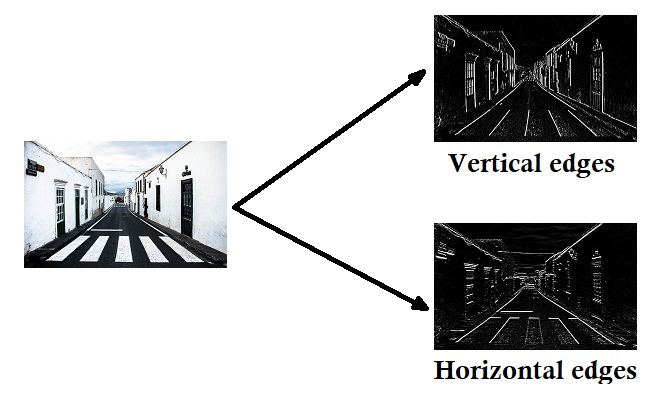
\includegraphics[width=1.\textwidth]{figures/edges.jpg}
\caption{Edge detected by different layers of a convolutional neural network.}
\label{fig:conv_filters}
\end{figure}

The CNN output won't be a single number but rather a list containing the probabilities that an image belongs to each class. Next we define the CNN architecture, see Fig.~\ref{fig:cnn2d}.

\begin{ipython}
import numpy as np, mnist
from keras.models import Sequential
from keras.layers import Dense, Conv2D, MaxPooling2D, Flatten
from tensorflow.keras.utils import to_categorical

train_images = mnist.train_images() 
train_labels = mnist.train_labels() 

model = Sequential()
model.add(Conv2D(8, kernel_size=3, input_shape=(28, 28, 1)))
model.add(MaxPooling2D(pool_size=2))
model.add(Flatten())
model.add(Dense(10, activation="softmax"))

model.compile(loss='categorical_crossentropy', optimizer='adam')
model.fit(train_images, to_categorical(train_labels), epochs=5, verbose=1)
\end{ipython}
\begin{ioutput}
Epoch 1/5
1875/1875 [==============================] - 19s 10ms/step - loss: 2.0868
Epoch 2/5
1875/1875 [==============================] - 18s 10ms/step - loss: 0.3320
Epoch 3/5
1875/1875 [==============================] - 18s 10ms/step - loss: 0.2153
Epoch 4/5
1875/1875 [==============================] - 18s 10ms/step - loss: 0.1891
Epoch 5/5
1875/1875 [==============================] - 18s 10ms/step - loss: 0.1799
<keras.callbacks.History at 0x7f07b05d0350>
\end{ioutput}

\begin{figure}[htb]
\centering
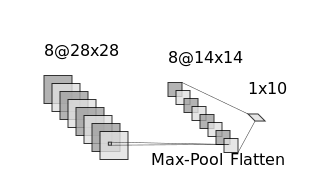
\includegraphics[width=0.9\textwidth]{figures/cnn_2d.png}
\caption{Graphical representation of the CNN developed to recognize handwritten digits.}
\label{fig:cnn2d}
\end{figure}

\begin{attention}
\subsubsection{Pooling}

Looking closely to the convolutional neural network implementation we can notice new kind of layers never used before, in particular the \texttt{MaxPooling2} layer.

Convolutional layers in a CNN systematically apply filters to input images in order to create feature maps that summarize the main characteristics of the sample.

A limitation of such maps is that they record the precise position of features in the input. This means that small movements in its position will result in a different feature map. This can happen with cropping, rotation, shifting, and other minor changes to the input image.

Imagine a program that looks for car plates in pictures taken by a speed radar: cars won't be in the same position in the frame so there may be differences in the classification of similar (but not equal) pictures.

A common approach to address this problem is called \emph{down sampling}. 
This is where a lower resolution version of an input signal (e.g. the picture) is created that still contains the large or important structural elements, without the finer detail that may not be as useful to the task.

Down sampling can be achieved using a pooling layer.
It involves selecting kind of a filter to be applied to the feature maps. The pooling operation size is smaller than the feature map; specifically, it is almost always 2×2 pixels. This means that the pooling layer will always reduce the size of each feature map by a factor of 2, e.g. each dimension is halved. For example, a pooling layer applied to a feature map of 6×6 (36 pixels) will result in an output pooled feature map of 3×3 (9 pixels).

The most common pooling operation are:
\begin{itemize}
\tightlist
\item Average Pooling: calculate the average value for each patch on the feature map;
\item Maximum Pooling (or Max Pooling): calculate the maximum value for each patch of the feature map.
\end{itemize}
\end{attention}

Let's see how well our NN predicts \texttt{mnist} testing digits.

\begin{ipython}
test_images = mnist.test_images()
test_labels = mnist.test_labels()

predictions = model.predict(test_images[:10])

print ("Tesing on MNIST digits...")
print("Predicted: ", np.argmax(predictions, axis=1)) 
print("Truth:     ", test_labels[:10])
\end{ipython}
\begin{ioutput}
Tesing on MNIST digits...
Predicted:  [7 2 1 0 4 1 4 4 6 9]
Truth: [7 2 1 0 4 1 4 9 5 9]
\end{ioutput}

Since the last but one digit has lower probability let's check the returned list to see which other number have non-zero probability.

\begin{ipython}
for i, p in enumerate(predictions[-2])])
    print("9th digit:", ["dig {}: {:.3f}".format(i, p)
\end{ipython}
\begin{ioutput}
9th digit: ['dig 0: 0.0000', 'dig 1: 0.0000', 'dig 2: 0.0000', 'dig 3: 0.0000', 
            'dig 4: 0.0000', 'dig 5: 0.0001', 'dig 6: 0.9999', 'dig 7: 0.0000', 
            'dig 8: 0.0000', 'dig 9: 0.0000']
\end{ioutput}

%So the second ranked digit is a 6 (which can be confused with a five if the lower loop is almost closed).

The NN performance can be checked using your own calligraphy. 

Open your favourite image editor (e.g. Paint, GIMP,\ldots) and create a black-white 200x200 pixels canvas. With the help of the mouse draw a digit and save it as a png file.
Before passing the image to the NN it has to be resized and this is done with an ad-hoc function, \texttt{transform\_image}, which can be imported from \href{https://raw.githubusercontent.com/matteosan1/finance_course/develop/libro/input_files/digit_converter.py}{\texttt{digit\_converter.py}}.

\begin{ipython}
from digit_converter import transform_image

filenames = ['four.png', 'five.png']
for f in filenames:
    test_images = np.array(transform_image(f))
test_images = np.expand_dims(test_images, axis=3)
predict = model.predict(test_images)

print ("Tesing on custom digits...")
print ("Predicted: ", np.argmax(predict, axis=1))
print("%:", ["{:.3f}".format(p[np.argmax(p)]) for p in predict])
print(["{:.2f}".format(p) for p in predict[0]])
\end{ipython}
\begin{ioutput}
Tesing on custom digits...
Predicted:  [4]
%: ['0.802']
['0.00', '0.00', '0.00', '0.00', '0.80', '0.00', '0.00', '0.20', '0.00', 
'0.00']

Testing on custom digits...
Predicted:  [5]
%: ['0.981']
['0.00', '0.00', '0.00', '0.01', '0.00', '0.98', '0.00', '0.01', '0.00', 
'0.00']
\end{ioutput}
The handwritten images used in this test are shown in Fig.~\ref{fig:test_images}.

\begin{figure}[htb]
\centering
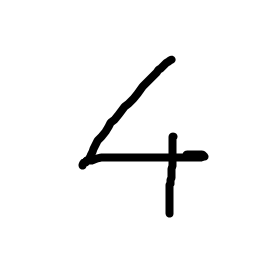
\includegraphics[width=0.2\textwidth]{figures/four.png}
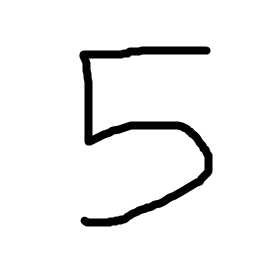
\includegraphics[width=0.2\textwidth]{figures/five.png}
\caption{Test handwritten digits used in the example.}
\label{fig:test_images}
\end{figure}

\section{Remarks on Artificial Intelligence}

A neural network is a \emph{black box} in the sense that while it can approximate any function, studying its structure won't give you any insights on the functional form of the function being approximated.

As an example, one common use of neural networks on the banking business is to classify loaners on "good payers" and "bad payers". You have a matrix of input characteristics $C$ (sex, age, income, etc) and a vector of results $R$ ("defaulted", "not defaulted", etc). When you model this using a neural network, you are supposing that there is a function $f(C)=R$, in the proper sense of a mathematical function. This function $f$ can be arbitrarily complex, and might change according to the evolution of the business, so you can't derive it by hand.

Then you use the Neural Network to build an approximation of $f$ that has an error rate that is acceptable to your application. This works, and the precision can be arbitrarily small, you can expand the network, fine tune its training parameters and get more data until the precision hits your goals.

The black box issue is: the approximation given by the neural network will not give you any insight on the form of $f$. There is no simple link between the weights and the function being approximated. 

Plus, from a traditional statistics viewpoint, a neural network is a non-identifiable model: given a dataset and network architecture, there can be two neural networks with different weights but exactly the same result. This makes the analysis very hard.
Needless to say, debugging NN results is even harder given this lack of interpretability. So use with caution machine learning models since they can be quite misleading.
 
\begin{thebibliography}{9}
\bibitem{bib:deep_learning} I. Goodfellow, Y. Bengio and A. Courville, \href{http://www.deeplearningbook.org}{\emph{Deep Learning}}, MIT Press, 2016
\bibitem{bib:nn_over_human}K. Grace, J. Salvatier, A. Dafoe, B. Zhang and O. Evans, \emph{When Will AI Exceed Human Performance? Evidence from AI Experts}, arXiv:1705.08807, 2005
\bibitem{bib:activation_function} J. Lederer, \emph{Activation Functions in Artificial Neural Networks: A Systematic Overview}, arxiv: 2101.09957, 2001
\bibitem{bib:backpropagation}\href{https://towardsdatascience.com/understanding-backpropagation-algorithm-7bb3aa2f95fd}{\emph{Understanding back-propagation algorithm}}, Towards Data Science [Online]
\bibitem{bib:loss_function}\href{https://medium.com/human-in-a-machine-world/mae-and-rmse-which-metric-is-better-e60ac3bde13d}{\emph{Mae and rmse which metric is better ?}}, Medium [Online]
\bibitem{bib:keras}\href{https://keras.io/}{\emph{Keras Documentation}}, [Online]  
\bibitem{bib:tensorflow}\href{https://www.tensorflow.org/}{\emph{Tensorflow Documentation}}, [Online] 
\bibitem{bib:scikit}\href{https://scikit-learn.org/stable/}{\emph{scikit-learn Documentation}}, [Online]
\end{thebibliography}